\section{Related Work}
\label{sec:related_work}

\begin{figure*}[t]
\centering
% --- Row 1 ---
\begin{subfigure}[b]{0.32\textwidth}
  \centering
  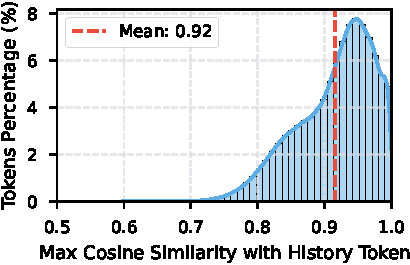
\includegraphics[width=\linewidth]{figures/visuals/insight_experiments/exp1_similarity_dist.pdf} 
  \caption{Token similarity.}
  \label{fig:token_sim_dist}
\end{subfigure}
\hfill
\begin{subfigure}[b]{0.32\textwidth} 
  \centering
  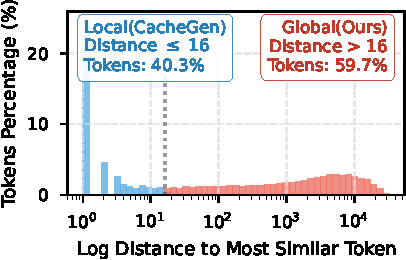
\includegraphics[width=\linewidth]{figures/visuals/insight_experiments/exp3_reference_distance_dist.pdf}
  \caption{Log distance to reference tokens.}
  \label{fig:distance_dist_to_sim_tokens}
\end{subfigure}
\hfill
\begin{subfigure}[b]{0.32\textwidth}
  \centering
  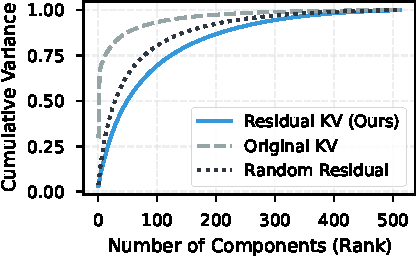
\includegraphics[width=\linewidth]{figures/visuals/insight_experiments/exp5_svd_variance.pdf}
  \caption{SVD analysis.}
  \label{fig:svd_analysis_of_token_cache}
\end{subfigure}
% --- Row 2 ---
\begin{subfigure}[b]{0.32\textwidth}
  \centering
  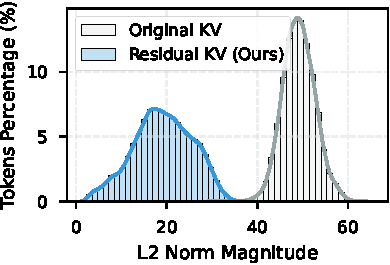
\includegraphics[width=\linewidth]{figures/visuals/insight_experiments/exp6_norm_dist.pdf}
  \caption{L2 Norm gap.}
  \label{fig:l2_norm_dist_gap}
\end{subfigure}
\hfill
\begin{subfigure}[b]{0.32\textwidth}
  \centering
  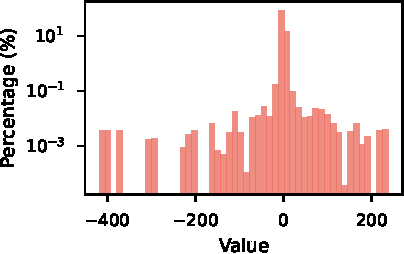
\includegraphics[width=\linewidth]{figures/visuals/comp_kv_range/raw_kv_global_dist.pdf}
  \caption{Original KV distribution.}
  \label{fig:raw_kv_range_dist}
\end{subfigure}
\hfill
\begin{subfigure}[b]{0.32\textwidth}
  \centering
  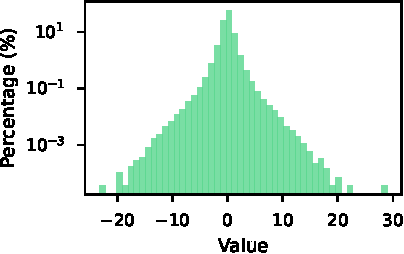
\includegraphics[width=\linewidth]{figures/visuals/comp_kv_range/ideal_res_global_dist.pdf}
  \caption{Residual KV distribution.}
  \label{fig:residual_kv_range_dist}
\end{subfigure}
% --- Main Caption ---
\caption{\textbf{Experimental analysis of KV redundancy and residualization.}}
% \caption{\textbf{Visualization of experimental analysis.} (a) Token similarity distribution. (b) Log distance distribution to most similar reference tokens. (c) SVD analysis of the original tokens' KV cache and the residual KV cache. (d) L2 Norm distribution gap between the original KV Cache and the residual KV cache. (e) Original KV value distribution. (f) Residual KV value distribution.}
\label{fig:combined_analysis_results}
\vspace{-1.0em}
\end{figure*}

As foundation models continue to scale, substantial effort has been devoted to reducing inference cost, enabling deployment under memory and latency constraints, and improving throughput~\cite{li2024snapkv, oren2024transformers_tova, liu2024intactkv, lin2025quantization, qi2025deltallm, liu2024deepseekv2, guo2025enhancing, hao2025tokenLRC}. 
Among these directions, the most relevant to our work are token selection, KV cache compression and quantization, token clustering, and inference frameworks for long-context LLMs.

\paragraph{Token Selection} 
Token selection methods aim to reduce attention cost by retaining only a subset of tokens.
%%%
They fall into \emph{static eviction} \cite{zhang2023h2o, oren2024transformers_tova, li2024snapkv, streamingllm}, which permanently remove tokens based on heuristics or early attention signals, and \emph{dynamic selection} \cite{hao2025omnikv, tang2024quest, zhang2025pqcache, xiao2024infllm, liu2025deepseek32, sun2024shadowkv}, which adaptively selects tokens during decoding. 
%%%
While dynamic methods achieve near-lossless accuracy in complex scenarios, they retain the full KV cache and rely on offloading, making performance bottlenecked by PCIe bandwidth. 
%%%
In contrast, DeltaKV performs GPU-resident, parallelizable compression that directly reduces KV cache footprint without offloading.


\paragraph{KV Cache Compression} 
KV cache compression methods exploit low-rank or subspace structure to reduce memory footprint \cite{saxena2024eigen, zhang2024lorc, chang2025palu, liu2024deepseekv2}, but typically require reconstructing the \emph{entire} KV cache during inference, incurring substantial computational overhead. 
%%%
DeltaKV instead compresses token-wise residuals relative to retrieved references and, when combined with sparse attention, reconstructs only $\le \mathbf{10\%}$ tokens, achieving significantly higher efficiency.


\paragraph{KV Cache Quantization} 
Quantization reduces memory and I/O cost by lowering numerical precision of KV caches, improving throughput in memory-bound decoding \cite{liu2024kivi, xiao2023smoothquant,hooper2024kvquant, he2024zipcache}. 
Yet, it neither reduces attention computation nor integrates well with sparsification due to channel-wise operations \cite{liu2024kivi}.
%%%
In contrast, DeltaKV produces low-magnitude residuals that naturally support token-level quantization for further memory reduction.


\paragraph{Token Clustering} 
Token clustering methods compress KV caches by reusing shared representations, but existing approaches either rely on CPU-hosted structures and incur PCIe bottlenecks (e.g., ClusterKV \cite{liu2025clusterkv}) or focus on local similarity, limiting reconstruction quality (e.g., Chelsea \cite{hu2025efficient_chelsea}). 
%%%
In contrast, DeltaKV performs global, GPU-resident residual compression using long-range similarity, avoiding external memory traffic.

\paragraph{Inference Frameworks}
Popular inference frameworks such as vLLM \cite{kwon2023efficient_vllm}, SGLang \cite{zheng2024sglang}, and LightLLM \cite{lightllm2} are optimized for full attention and page-based KV management, making sparsification and compression difficult to integrate. 
%%%
Recent adaptations either sacrifice batch scalability (e.g., Sparse Frontier~\cite{nawrot2025sparsefrontier}) or rely on less optimized backends (e.g., KVPress~\cite{devoto2025expectedattention_kvpress}).
%%%
In contrast, Sparse-vLLM abandons page-level assumptions and natively supports sparse, irregular KV layouts, enabling efficient deployment of DeltaKV in practice.


